\centering
%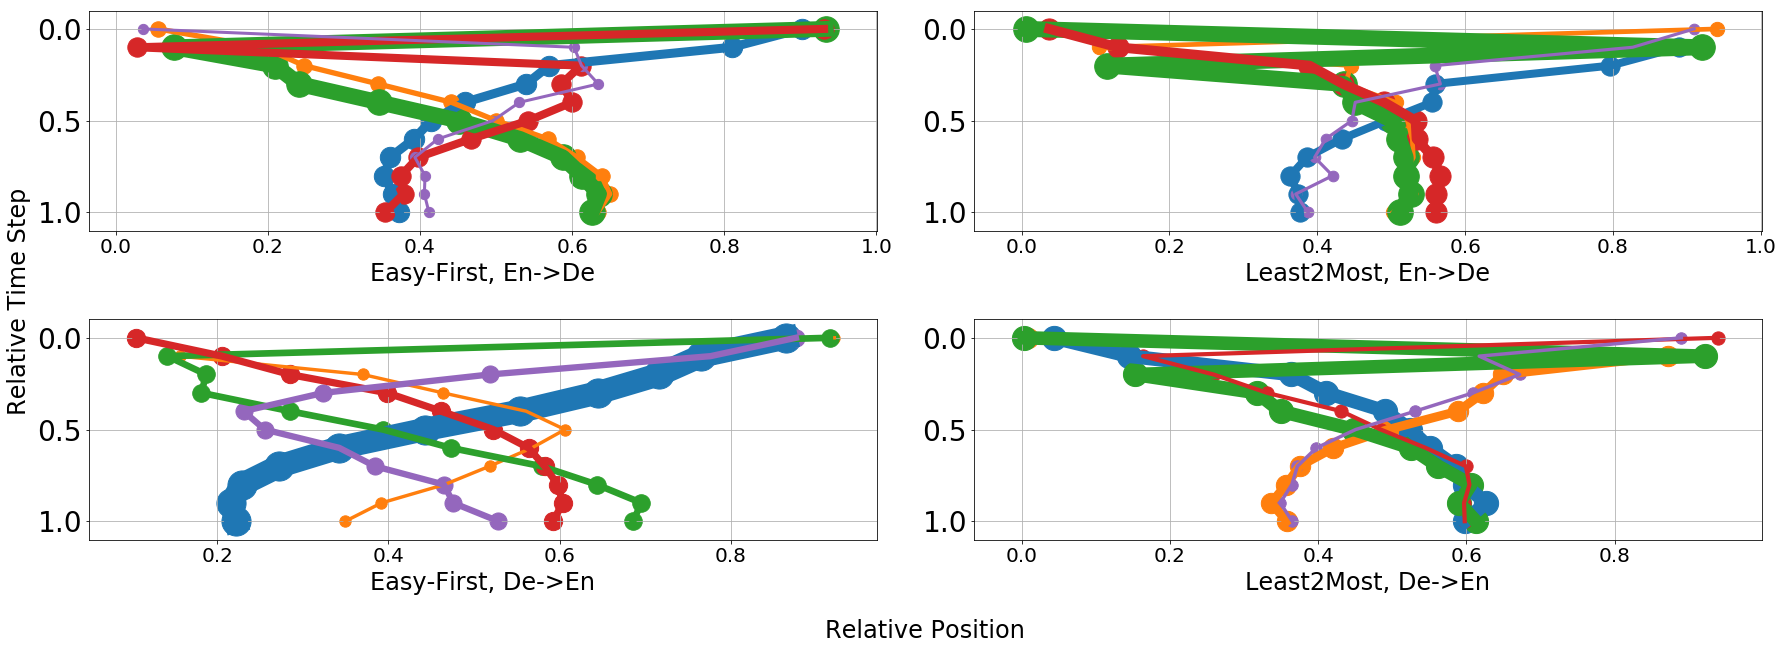
\includegraphics[width=\textwidth]{figures/all-position-clusters.png}
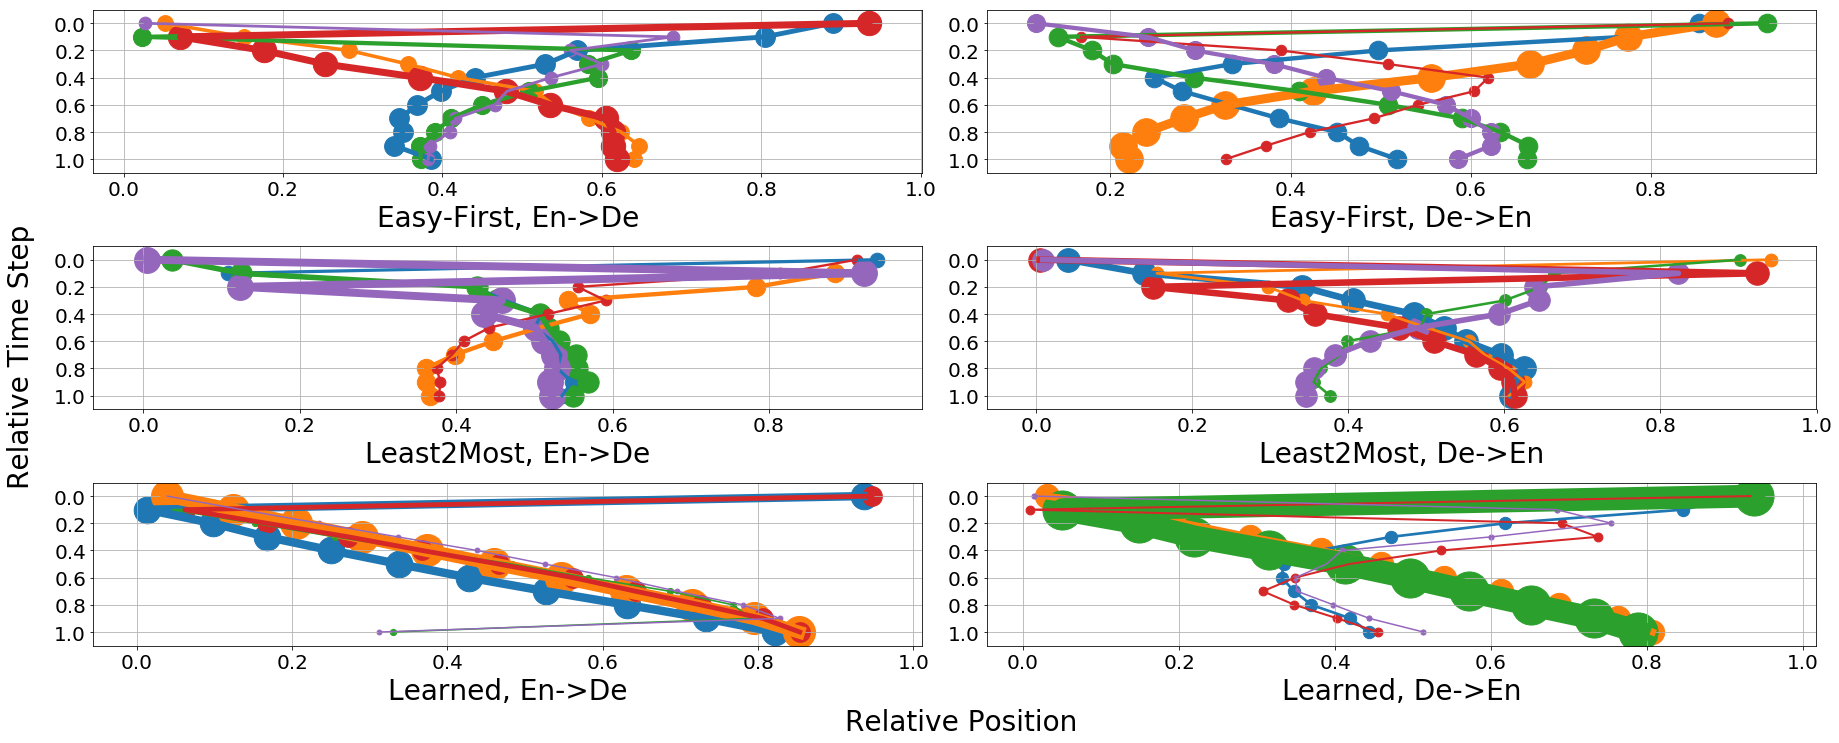
\includegraphics[width=\textwidth]{figures/pos-plot.png}
%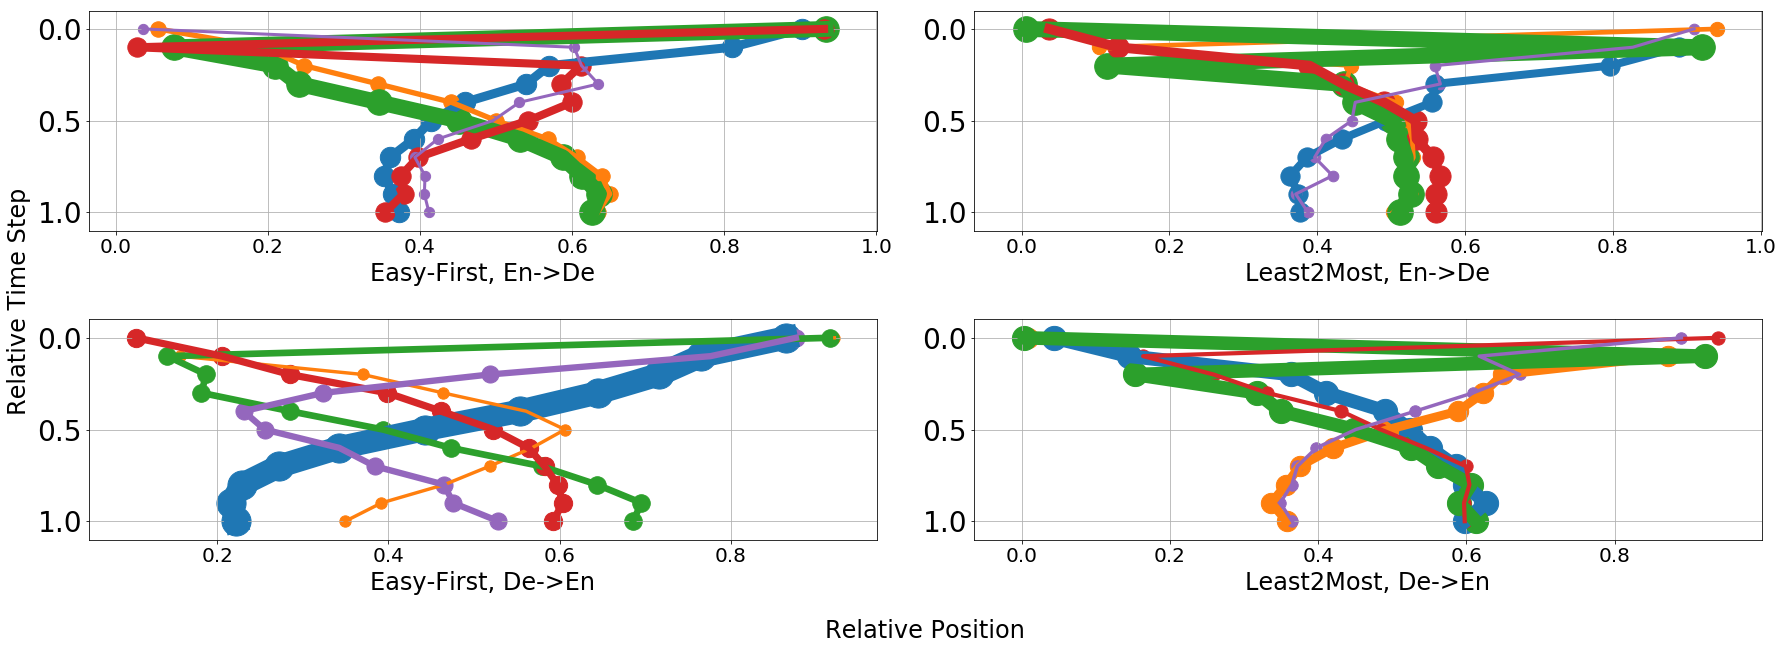
\includegraphics[width=\columnwidth,clip=true,trim=0 50 0 0]{figures/all-position-clusters.png}

%\begin{subfigure}[t]{0.49\textwidth}
%    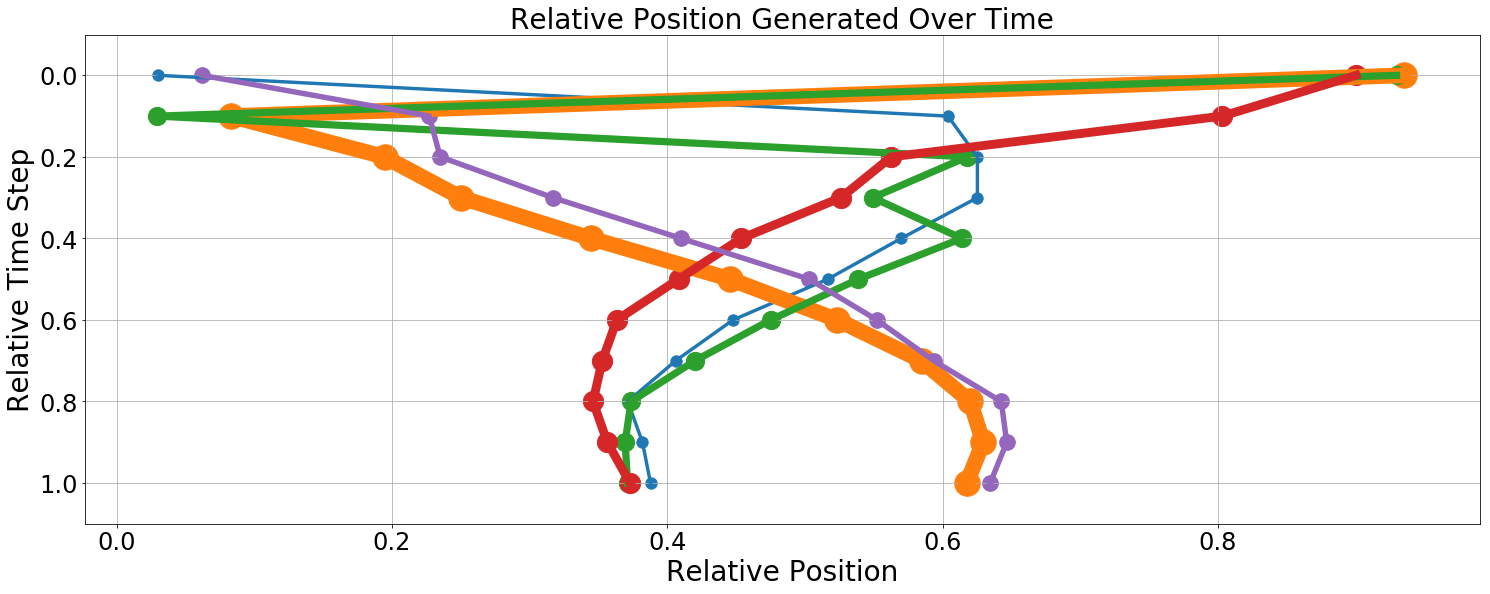
\includegraphics[width=\columnwidth]{figures/ef-en-de.png}
%    \caption{Easy First on En$\rightarrow$De}
%\end{subfigure}
%~
%\begin{subfigure}[t]{0.49\textwidth}
%    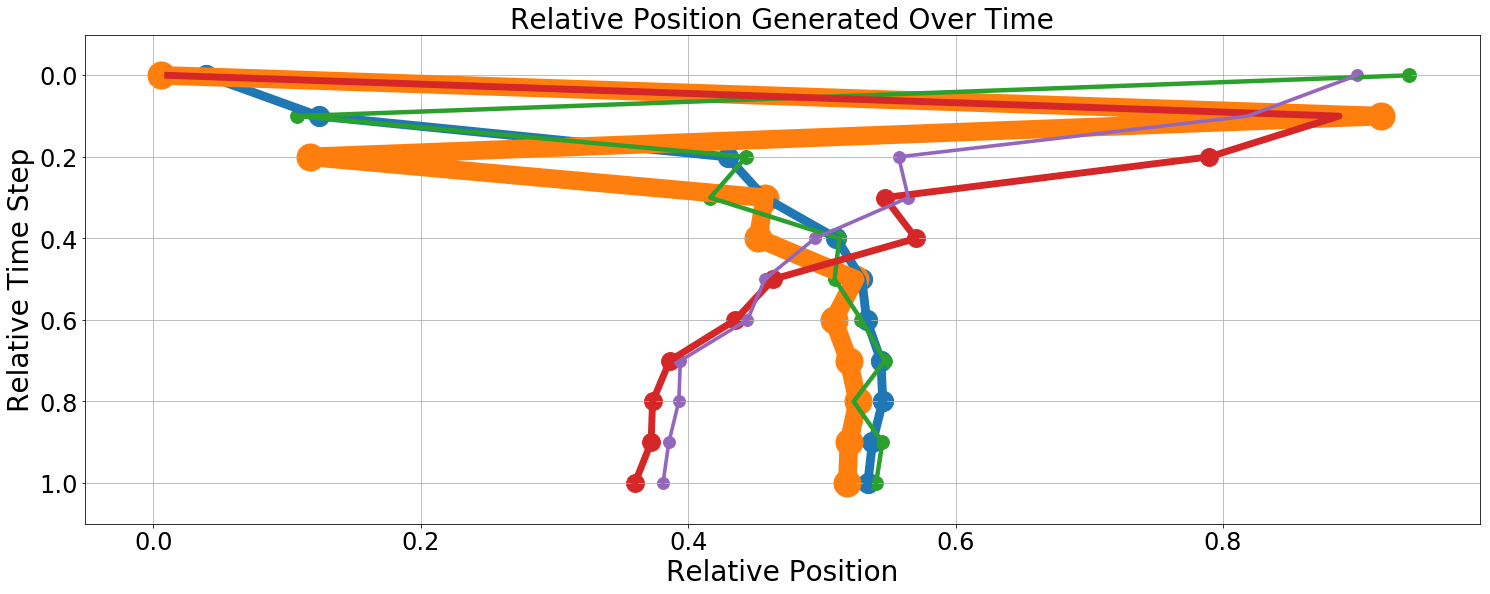
\includegraphics[width=\columnwidth]{figures/lm-en-de.png}
%    \caption{Least-to-Most on En$\rightarrow$De}
%\end{subfigure}
%\begin{subfigure}[t]{0.49\textwidth}
%    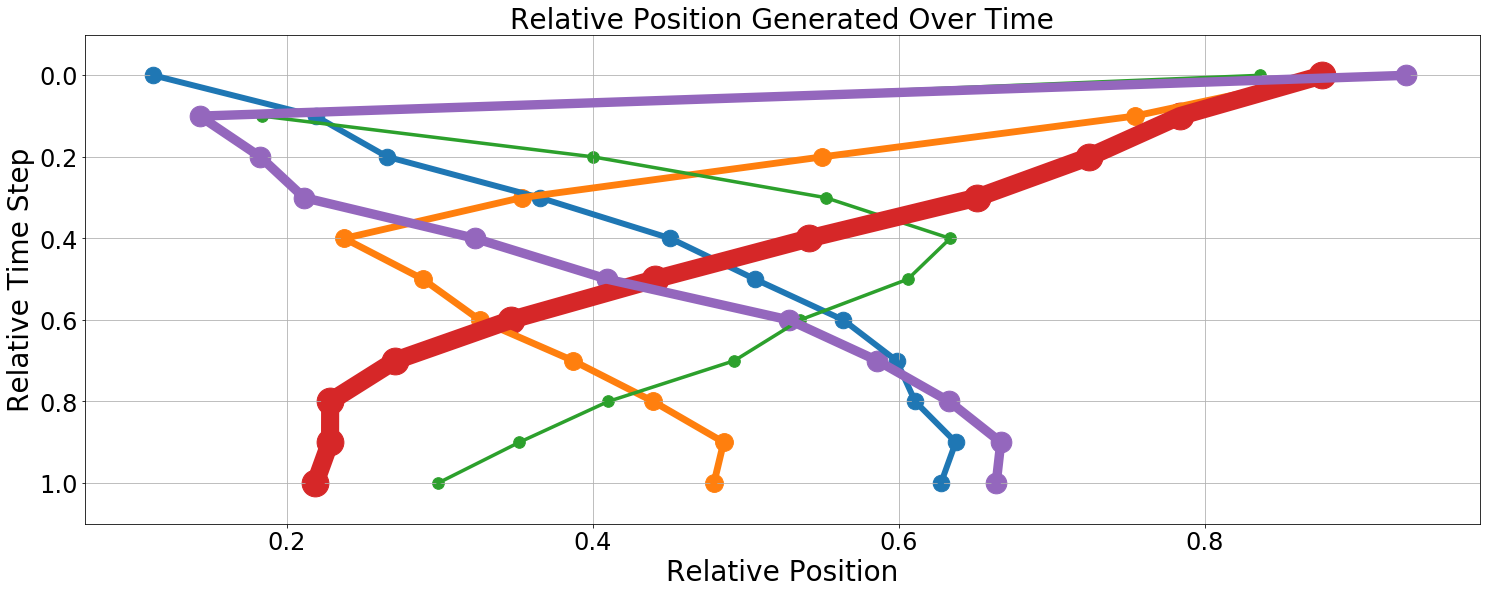
\includegraphics[width=\columnwidth]{figures/ef-de-en.png}
%    \caption{Easy First on De$\rightarrow$En}
%\end{subfigure}
%~
%\begin{subfigure}[t]{0.49\textwidth}
%    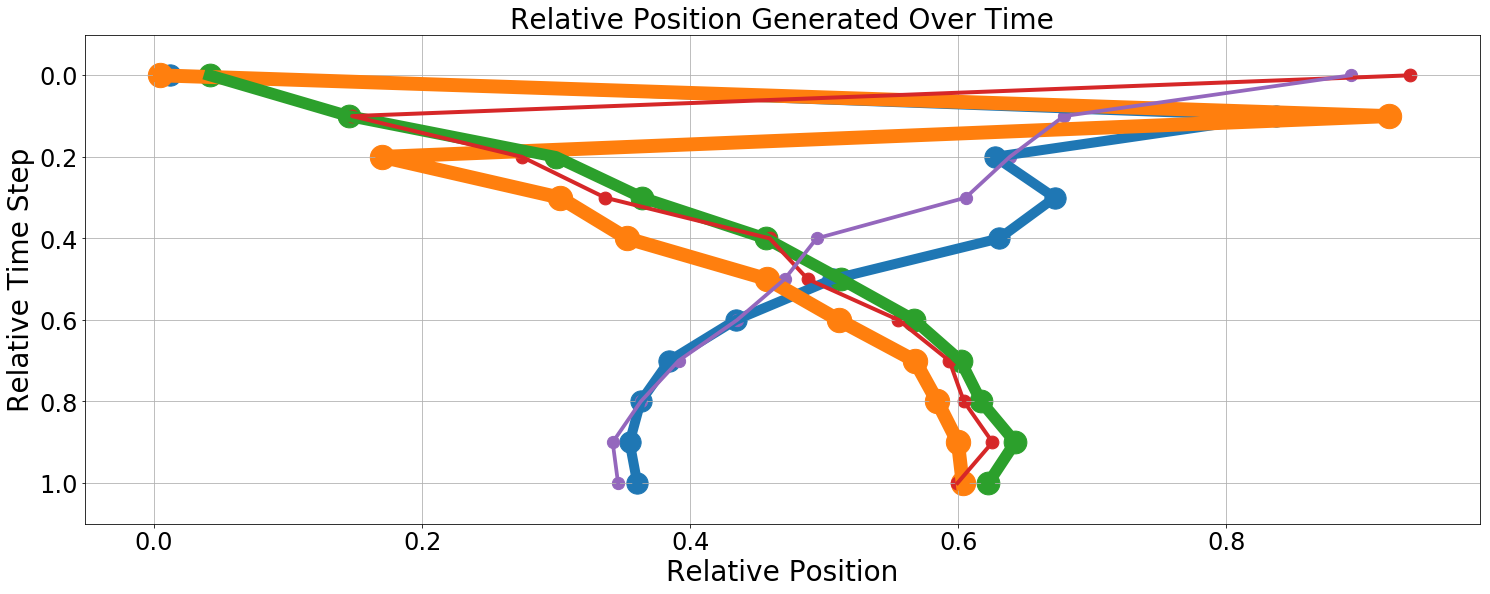
\includegraphics[width=\columnwidth]{figures/lm-de-en.png}
%    \caption{Least-to-Most on De$\rightarrow$En}
%\end{subfigure}
\caption{Generation orders given by {\bf easy-first}, {\bf least2most}, and {\bf learned} coordinate selection. 
We use greedy search with $L$ iterations on the development set.
We group the orders into five clusters using and visualize cluster centers with normalized positions (x-axis) over normalized generation steps (y-axis).
The thickness of a line is proportional to the number of examples in the corresponding cluster.}